\documentclass{article}

\usepackage[utf8]{inputenc}
\usepackage[margin=1in]{geometry}
\usepackage{amsfonts, amsmath, amssymb, amsthm}
\usepackage{setspace}
\usepackage{enumitem}
\usepackage{graphicx}
\usepackage{multicol}
\RequirePackage{pinlabel}

\usepackage{xcolor}
\usepackage{soul}

\setlength{\parindent}{0pt}
\onehalfspacing

% Please excuse my LaTeX code.

\begin{document}
MATH 241 | FALL 2024

\vspace{1in}

\begin{center}
\LARGE{Midterm 1 }
\end{center}

\vspace{0.5in}

\begin{center}
Name (Last, First): \underline{\hspace{3in}} \qquad Section: \underline{\hspace{1in}}
\end{center}

\vspace{0.5in}

\begin{center}
\begin{tabular}{ |c|c|c|c|c|c|c|c|c|c| }
\hline
Question: & 1 & 2 & 3 & 4 & 5 & 6 & 7 & 8 & Total \\
\hline
Points: & 6 & 8 & 20 & 20 & 6 & 20 & 8 & 12 & 100 \\
\hline
Score: & \hspace{0.25in} & \hspace{0.25in} & \hspace{0.25in} & \hspace{0.25in} & \hspace{0.25in} & \hspace{0.25in} & \hspace{0.25in} & \hspace{0.25in} & {} \\
\hline
\end{tabular}
\end{center}

\vspace{0.5in}

\begin{large}
\textbf{Instructions}:

\begin{itemize}
\item Write your full name (last, first) and section number above.
\item Answer all the questions below and show your work.
\item No electronic devices are to be used during the exam (this includes calculators).
\item The exam is closed book and closed notes.
\item \textbf{Do not use L'H\^{o}pital's rule anywhere on this exam}.
\item Turn in your exam at the end of the period.
\end{itemize}

Good luck!
\end{large}

\vspace{1in}

\textbf{Sign below to acknowledge that you have read and agree to the above instructions.}

\vspace{0.5cm}

\noindent Signature: \underline{\hspace{5in}}

\pagestyle{empty}

\newpage

\pagestyle{plain}

\section*{Question 1 (6 points)}
The domain of the functions $f$ and $g$ is the closed interval $[0,4]$ and their graphs are represented below.
\begin{figure}[h!]
	\labellist
	\small
	\pinlabel $f(x)$ at 108 140
	\pinlabel $g(x)$ at 123 115
	\endlabellist
	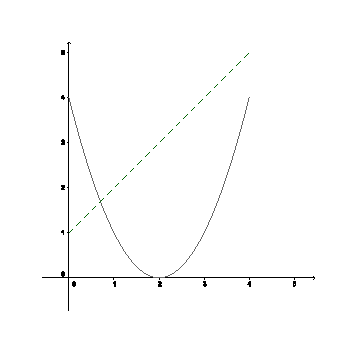
\includegraphics[width=0.6
\textwidth]{1-3-01}
\end{figure}

Determine whether the following compositions are defined. When they are defined, determine their value.

 \begin{enumerate}[label=(\alph*)]
    \item (2 points) $(f\circ g)(2)$
    \vspace{1in}
    \item (2 points) $(g\circ g)(2)$
    \vspace{1in}
    \item (2 points) $(f\circ f)(4)$
    \end{enumerate}


\pagebreak

\section*{Question 2 (8 points)}
Consider the function
$$f(x)=\frac{1}{x^2-2x-3}.$$


\begin{enumerate}[label=(\alph*)]
    \item  (2 points) What is the domain of $f$?
    \vspace{1in}

    \item (4 points) Find all numbers $a$ such that the vertical line $x=a$ is a vertical asymptote of the curve $y=f(x)$. In each case, indicate if the limit \textbf{from the right} is $\infty$ or $-\infty$.
    \vspace{3in}
    \item (2 points) If $g(x)=\frac{1}{x^2-4}$, what transformation takes the graph of $g$ to the graph of $f$? 

    (\textit{Hint:} Note that $x^2-2x-3= (x-1)^2-4$.)

\end{enumerate}

\pagebreak

\section*{Question 3 (20 points)}
Find each of the following limit, if it exists. If it does not exist and if the limit is infinite, state whether it is $-\infty$ or $\infty$.

    \begin{enumerate}[label=(\alph*)]
        \item (5 points) $\displaystyle \lim_{x \to 4} \frac{\sqrt{x}-2}{x-4}$.
        \vspace{1.5in}
        \item (5 points) $\displaystyle \lim_{x \to 0} x \operatorname{cot} x$.
        \vspace{1.5in}
        \item (5 points) $\displaystyle \lim_{x \to 0} (\sqrt{x^2+x})\sin{\left(\frac{1}{x}\right)}$.
        \vspace{2in}
        \item (5 points) $\displaystyle \lim_{x \to -2} \frac{2-|x|}{2+x}$.
        \vspace{2in}
    \end{enumerate}

\pagebreak

\section*{Question 4 (20 points)}
Let $\displaystyle f(x) =\sqrt{2x+1}$.

    \begin{enumerate}[label=(\alph*)]
    \item (2 points) Write down the expression for $f'(x)$ as a limit.
    \vspace{0.5in}
    \item (8 points) Calculate this limit to show that $f'(x)=\frac{1}{\sqrt{2x+1}}$.
    \vspace{4in}
    \item (4 points) What is the domain of the function $f'$ from part (b)?
    \vspace{0.5in}
    \item (6 points) Use part (b) to find the equation of the tangent line to the curve $y=f(x)$ at the point $(0,1)$.

    \end{enumerate}

\pagebreak

\section*{Question 5 (6 points)}
Consider the function $f$ defined by
\begin{displaymath}
f(x) = \left\{ \begin{array}{ll}
-x & \textrm{if $x<-1$}\\
\sin{\left(\frac{\pi}{2}x\right)} & \textrm{if $-1 \leq x <1 $}\\
2 & \textrm{if $x=1$}\\
2-x & \textrm{if $x>1$}\\
\end{array} \right.
\end{displaymath}

        \begin{enumerate}[label=(\alph*)]
            \item (2 points) Sketch the graph of $f$.

            \vspace{1cm}
            \begin{center}
            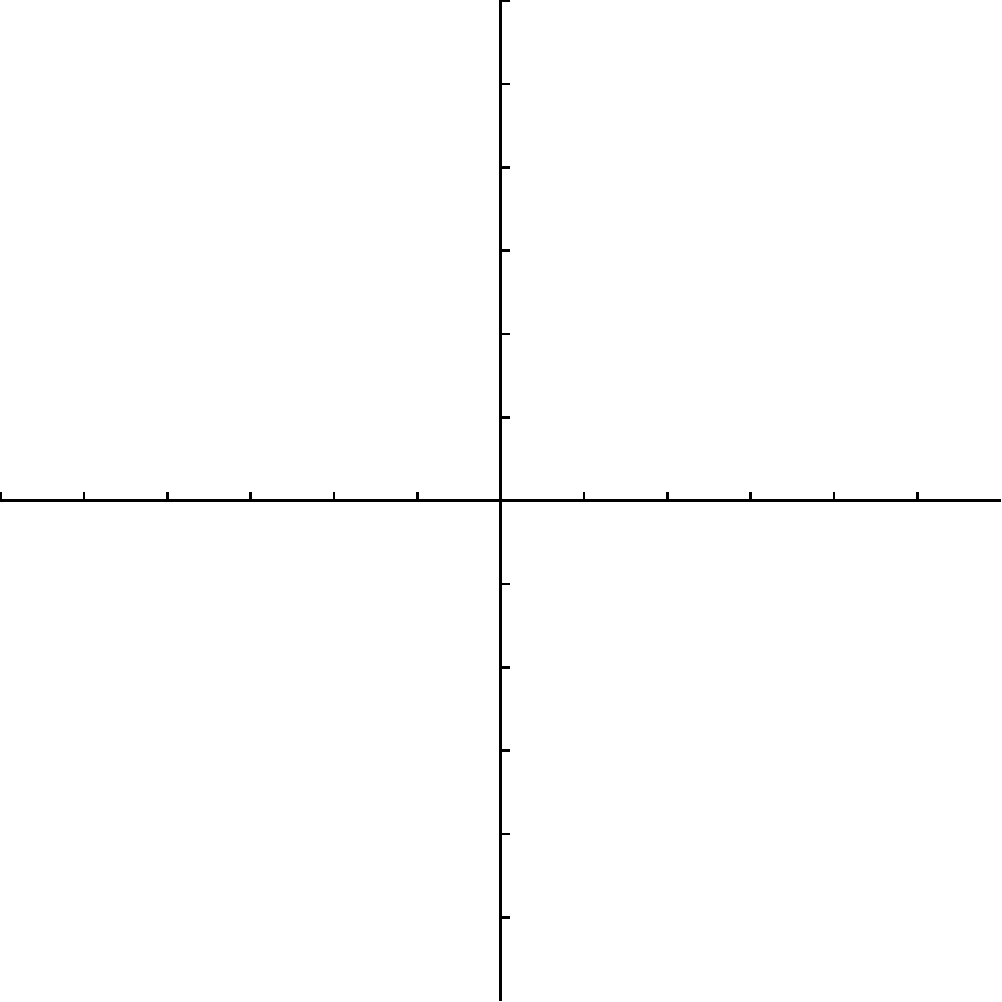
\includegraphics[width=0.5\textwidth]{blank.pdf}
            \end{center}
            \vspace{\fill}
            \item (2 points) Find the values $a$ such that
                $\displaystyle\lim_{x\to a}{f(x)}$ does not exist.
                \vspace{\fill}
            \item (2 points) Find the values $a$ such that $f(x)$ is
                discontinuous at $x=a$.
                \vspace{\fill}

        \end{enumerate}

\pagebreak

\section*{Question 6 (20 points)}
In each of the following, find the derivative $\frac{dy}{dx}$. You should simplify as much as possible, but do not waste too much time doing it.


    \begin{enumerate}[label=(\alph*)]
        \item (5 points) $y=\left( \sqrt{x}+\frac{1}{x} \right)^5$.
        \vspace{1.5in}
        \item (5 points) $y= x^2 \sin{\sqrt{x}}$.
        \vspace{2in}
        \item (5 points) $y=x^{3/2}+\sqrt{x}$.
        \vspace{1.5in}
        \item (5 points) $x^3-3x^2y+2xy^2=0$.

        (\textit{Hint}: Use implicit differentiation. You can give your answer as an expression in $x$ and $y$.)

    \end{enumerate}

\pagebreak





\section*{Question 7 (8 points)}
The height (in meters) of a projectile shot vertically upward from a point $2$ m above ground level with an initial velocity of $2$ m/s is $s(t)=2+2t-4.9t^2$ after $t$ seconds.

    \begin{enumerate}[label=(\alph*)]
        \item (4 points) Find the velocity after $4$ seconds.
        \vspace{3in}
        \item (4 points) What is the maximum height? You can give your answer in the form of a fraction.

        (\textit{Hint:} At maximum height, the velocity is zero.)
    \end{enumerate}

\pagebreak

\section*{Question 8 (12 points)}
A snowball melts so that its surface area decreases at a rate of $1 \, \operatorname{cm}^2/\operatorname{min}$. Find the rate at which the diameter decreases when the radius is $5 \, \operatorname{cm}$.

(\textit{Hint}: Recall that the surface area of a sphere of radius $r$ is $4 \pi r^2$.)


\end{document}